\documentclass[a4paper,11pt]{article}
\usepackage{a4wide}
\usepackage{fullpage}
\usepackage[utf8x]{inputenc}
%\usepackage[slovene]{babel}
%\selectlanguage{slovene}
\usepackage[toc,page]{appendix}
\usepackage[pdftex]{graphicx} 
\usepackage{amsfonts}
\usepackage{amsmath}
\usepackage{setspace}
\usepackage{color}
\definecolor{light-gray}{gray}{0.95}
\usepackage{listings} 
\usepackage{hyperref}
\renewcommand{\baselinestretch}{1.2} 
\renewcommand{\appendixpagename}{Priloge}

\lstset{ 
language=Python,
basicstyle=\footnotesize,
basicstyle=\ttfamily\footnotesize\setstretch{1},
backgroundcolor=\color{light-gray},
}

\title{Topological data analysis \\ Homework 3}
\author{Sara Bizjak (27202020)}
\date{\today}

\begin{document}

\maketitle

%%%%%%%%%%%%%%%%%%%%%%%%%%%%%%%%%%%%%%%%%%%%%%%%%%%%%%%%%%%%%%%%%%%%%%%%%%%%%%%%%%%%%%%%%%%%%%%%%%%%%%%%%%%%%%%%%%%%%%%%%%%%%%%%%%%%%%%%%%%%%%%%%%%%%%%%%%%%%%%%

\section{Theoretical problems}
\subsection{Homology}
For the simplicial complex $X$:

\begin{figure}[ht!]
    \centering
    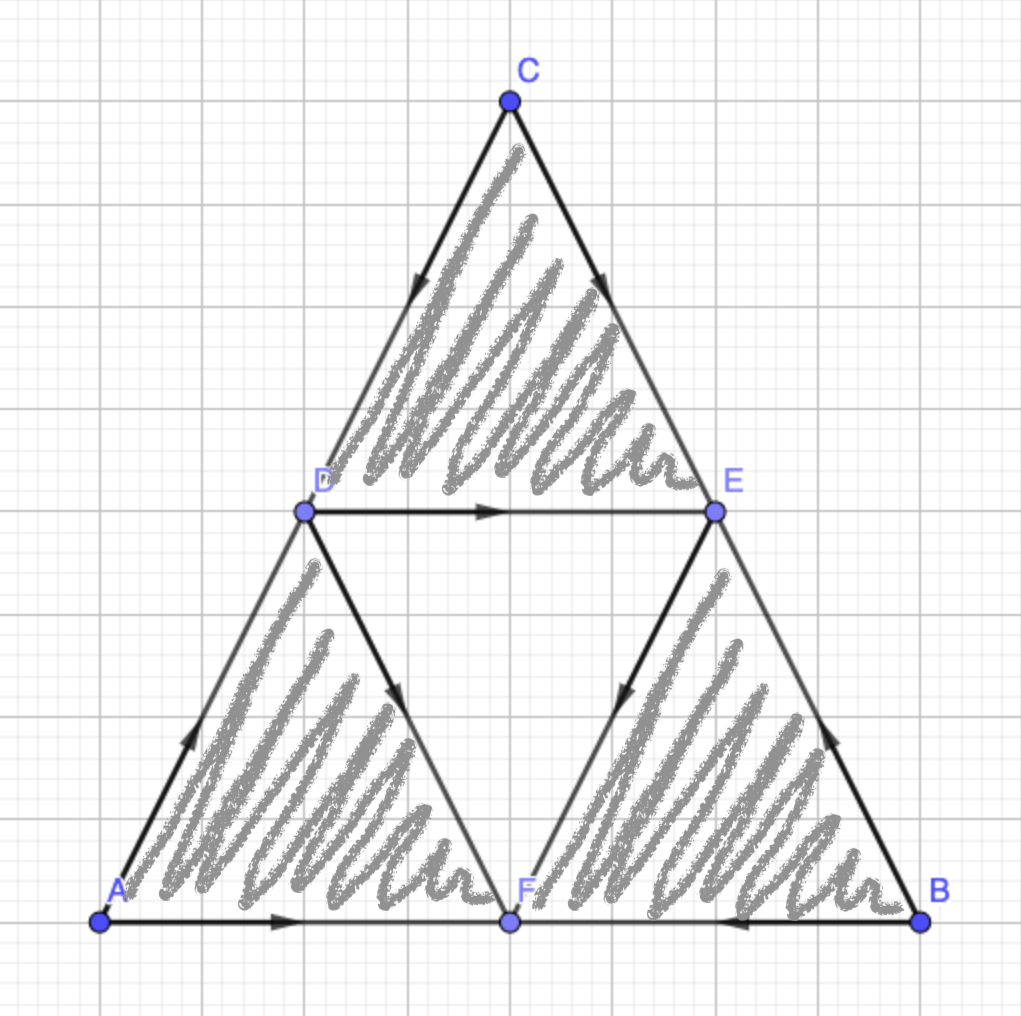
\includegraphics[width=80mm]{1a.png}
    \caption{Simplicial complex $X$.}
\end{figure}

%%%%%%%%%%%%%%%%%%%%%%%%%%%%%%
%%%%%%%%%%%%%%%%%%%%%%%%%%%%%%
\noindent
a) Write the chain groups $C_n$.
\\
$$ 
c_0 = \langle A, B, C, D, E, F \rangle,
$$
$$
c_1 = \langle AD, AF, BE, BF, CD, CE, DE, DF, EF \rangle,
$$
$$
c_2 = \langle ADF, BEF, CDE \rangle.
$$
%%%%%%%%%%%%%%%%%%%%%%%%%%%%%%
%%%%%%%%%%%%%%%%%%%%%%%%%%%%%%
b) Determine the boundary homomorphism $\partial_n : C_n \rightarrow C_{n - 1}$.
\\
We have
$$
\partial_2(ADF) = AD + DF - AF,
$$
$$
\partial_2(CDE) = CD + DE - CE,
$$
$$
\partial_2(BEF) = BE + EF - BF,
$$
$$
\partial_1(AD) = D - A,
$$
$$
\partial_1(AF) = F - A,
$$
$$
\partial_1(BE) = E - B,
$$
$$
\partial_1(BF) = F - B,
$$
$$
\partial_1(CD) = D - C,
$$
$$
\partial_1(CE) = E - C,
$$
$$
\partial_1(DE) = E - D,
$$
$$
\partial_1(DF) = F - D,
$$
$$
\partial_1(EF) = F - E,
$$
$$
\partial_0(A) = \partial_0(B) = \partial_0(C) = \partial_0(D) = \partial_0(E) = \partial_0(F) = 0.
$$
%%%%%%%%%%%%%%%%%%%%%%%%%%%%%%
%%%%%%%%%%%%%%%%%%%%%%%%%%%%%%
c) Find the cycles $Z_n = ker \partial_n.$
\\
There are no cycles for $ n = 2 $ because $X$ only has three 2-simplexes (we need at least four).
$$
Z_2 = ker \partial_2 = \langle 0 \rangle,
$$
$$
Z_1 = ker \partial_1 = \langle AD + DF - AF, BE + EF - BF, CD + DE - CE, DE + EF - DF \rangle,
$$
$$
Z_0 = ker \partial_0 = \langle A, B, C, D, E, F \rangle.
$$
%%%%%%%%%%%%%%%%%%%%%%%%%%%%%%
%%%%%%%%%%%%%%%%%%%%%%%%%%%%%%
d) Find the boundaries $B_n = im \partial_n$.
$$
B_2 = im \partial_3 = \langle 0 \rangle,
$$
$$
B_1 = im \partial_2 = \langle AD + DF - AF, BE + EF - BF, CD + DE - CE \rangle,
$$
$$
B_0 = im \partial_1 = \langle D - A, F - A, E - B, F - B, D - C, E - C, E - D, F - D, F - E \rangle.
$$
%%%%%%%%%%%%%%%%%%%%%%%%%%%%%%
%%%%%%%%%%%%%%%%%%%%%%%%%%%%%%
e) Determine the homology groups with $\mathbb{Z}$ coefficients, $H_n(X;\mathbb{Z})$.
$$
H_2(X;\mathbb{Z}) = \frac{Z_2}{B_2} = \frac{\langle 0 \rangle}{\langle 0 \rangle} = \langle 0 \rangle,
$$
\begin{align*}
H_1(X;\mathbb{Z}) &= \frac{Z_1}{B_1} = \frac{\langle AD + DF - AF, BE + EF - BF, CD + DE - CE, DE + EF - DF \rangle}{\langle AD + DF - AF, BE + EF - BF, CD + DE - CE \rangle} 
\\
&= \langle DE + EF - DF \rangle = \mathbb{Z},
\end{align*}
\begin{align*}
H_0(X;\mathbb{Z}) &= \frac{Z_0}{B_0} = \frac{\langle A, B, C, D, E, F \rangle}{\langle D - A, F - A, E - B, F - B, D - C, E - C, E - D, F - D, F - E \rangle} 
\\
&= \langle A \rangle = \mathbb{Z}.
\end{align*}
%%%%%%%%%%%%%%%%%%%%%%%%%%%%%%
%%%%%%%%%%%%%%%%%%%%%%%%%%%%%%
f) Determine the homology groups with $\mathbb{Z}_2$ coefficients, $H_n(X;\mathbb{Z}_2)$.
$$
H_2(X;\mathbb{Z}_2) = \frac{Z_2}{B_2} = \frac{\langle 0 \rangle}{\langle 0 \rangle} = \langle 0 \rangle,
$$
\begin{align*}
H_1(X;\mathbb{Z}_2) &= \frac{Z_1}{B_1} = \frac{\langle AD + DF + AF, BE + EF + BF, CD + DE + CE, DE + EF + DF \rangle}{\langle AD + DF + AF, BE + EF + BF, CD + DE + CE \rangle} 
\\
&= \langle DE + EF + DF \rangle = \mathbb{Z}_2,
\end{align*}
\begin{align*}
H_0(X;\mathbb{Z}_2) &= \frac{Z_0}{B_0} = \frac{\langle A, B, C, D, E, F \rangle}{\langle D + A, F + A, E + B, F + B, D + C, E + C, E + D, F + D, F + E \rangle} 
\\
&= \langle A \rangle = \mathbb{Z}_2.
\end{align*}
%%%%%%%%%%%%%%%%%%%%%%%%%%%%%%
%%%%%%%%%%%%%%%%%%%%%%%%%%%%%%
g) Determine the Betti numbers of X.
\\
The Betti number of $X$ are $b_2 = 0$, $b_1 = 1$, $b_0 = 1$.
\\
%%%%%%%%%%%%%%%%%%%%%%%%%%%%%%
%%%%%%%%%%%%%%%%%%%%%%%%%%%%%%
h) Determine the Euler characteristics of $X$.
\\
$\chi(X) = b_0 - b_1 + b_2 = 1 - 1 + 0 = 0$.

%%%%%%%%%%%%%%%%%%%%%%%%%%%%%%%%%%%%%%%%%%%%%%%%%%%%%%%%%%%%
%%%%%%%%%%%%%%%%%%%%%%%%%%%%%%%%%%%%%%%%%%%%%%%%%%%%%%%%%%%%
%%%%%%%%%%%%%%%%%%%%%%%%%%%%%%%%%%%%%%%%%%%%%%%%%%%%%%%%%%%%
%%%%%%%%%%%%%%%%%%%%%%%%%%%%%%%%%%%%%%%%%%%%%%%%%%%%%%%%%%%%
%%%%%%%%%%%%%%%%%%%%%%%%%%%%%%%%%%%%%%%%%%%%%%%%%%%%%%%%%%%%

\subsection{Homology}
For the simplicial complex $X$:

\begin{figure}[ht!]
    \centering
    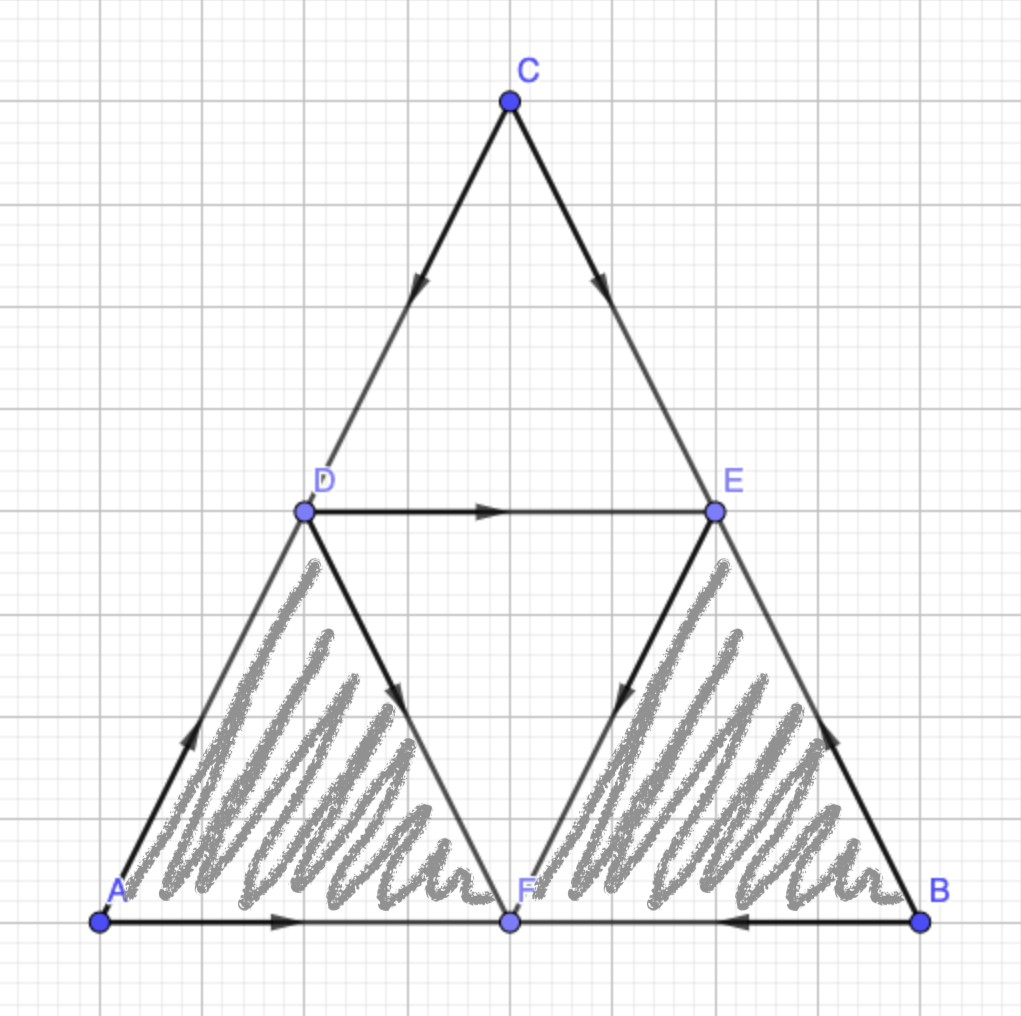
\includegraphics[width=80mm]{1b.png}
    \caption{Simplicial complex $X$.}
\end{figure}

%%%%%%%%%%%%%%%%%%%%%%%%%%%%%%
%%%%%%%%%%%%%%%%%%%%%%%%%%%%%%
\noindent
a) Write the chain groups $C_n$.
\\
$$ 
c_0 = \langle A, B, C, D, E, F \rangle,
$$
$$
c_1 = \langle AD, AF, BE, BF, CD, CE, DE, DF, EF \rangle,
$$
$$
c_2 = \langle ADF, BEF \rangle.
$$
%%%%%%%%%%%%%%%%%%%%%%%%%%%%%%
%%%%%%%%%%%%%%%%%%%%%%%%%%%%%%
b) Determine the boundary homomorphism $\partial_n : C_n \rightarrow C_{n - 1}$.
\\
We have
$$
\partial_2(ADF) = AD + DF - AF,
$$
$$
\partial_2(BEF) = BE + EF - BF,
$$
$$
\partial_1(AD) = D - A,
$$
$$
\partial_1(AF) = F - A,
$$
$$
\partial_1(BE) = E - B,
$$
$$
\partial_1(BF) = F - B,
$$
$$
\partial_1(CD) = D - C,
$$
$$
\partial_1(CE) = E - C,
$$
$$
\partial_1(DE) = E - D,
$$
$$
\partial_1(DF) = F - D,
$$
$$
\partial_1(EF) = F - E,
$$
$$
\partial_0(A) = \partial_0(B) = \partial_0(C) = \partial_0(D) = \partial_0(E) = \partial_0(F) = 0.
$$
%%%%%%%%%%%%%%%%%%%%%%%%%%%%%%
%%%%%%%%%%%%%%%%%%%%%%%%%%%%%%
c) Find the cycles $Z_n = ker \partial_n.$
$$
Z_2 = ker \partial_2 = \langle 0 \rangle,
$$
$$
Z_1 = ker \partial_1 = \langle AD + DF - AF, BE + EF - BF, CD + DE - CE, DE + EF - DF \rangle,
$$
$$
Z_0 = ker \partial_0 = \langle A, B, C, D, E, F \rangle.
$$
%%%%%%%%%%%%%%%%%%%%%%%%%%%%%%
%%%%%%%%%%%%%%%%%%%%%%%%%%%%%%
d) Find the boundaries $B_n = im \partial_n$.
$$
B_2 = im \partial_3 = \langle 0 \rangle,
$$
$$
B_1 = im \partial_2 = \langle AD + DF - AF, BE + EF - BF \rangle,
$$
$$
B_0 = im \partial_1 = \langle D - A, F - A, E - B, F - B, D - C, E - C, E - D, F - D, F - E \rangle.
$$
%%%%%%%%%%%%%%%%%%%%%%%%%%%%%%
%%%%%%%%%%%%%%%%%%%%%%%%%%%%%%
e) Determine the homology groups with $\mathbb{Z}$ coefficients, $H_n(X;\mathbb{Z})$.
$$
H_2(X;\mathbb{Z}) = \frac{Z_2}{B_2} = \frac{\langle 0 \rangle}{\langle 0 \rangle} = \langle 0 \rangle,
$$
\begin{align*}
H_1(X;\mathbb{Z}) &= \frac{Z_1}{B_1} = \frac{\langle AD + DF - AF, BE + EF - BF, CD + DE - CE, DE + EF - DF \rangle}{\langle AD + DF - AF, BE + EF - BF \rangle} 
\\
&= \langle CD + DE - CE, DE + EF - DF \rangle = \mathbb{Z} \oplus \mathbb{Z},
\end{align*}
\begin{align*}
H_0(X;\mathbb{Z}) &= \frac{Z_0}{B_0} = \frac{\langle A, B, C, D, E, F \rangle}{\langle D - A, F - A, E - B, F - B, D - C, E - C, E - D, F - D, F - E \rangle} 
\\
&= \langle A \rangle = \mathbb{Z}.
\end{align*}
%%%%%%%%%%%%%%%%%%%%%%%%%%%%%%
%%%%%%%%%%%%%%%%%%%%%%%%%%%%%%
f) Determine the homology groups with $\mathbb{Z}_2$ coefficients, $H_n(X;\mathbb{Z}_2)$.
$$
H_2(X;\mathbb{Z}_2) = \frac{Z_2}{B_2} = \frac{\langle 0 \rangle}{\langle 0 \rangle} = \langle 0 \rangle,
$$
\begin{align*}
H_1(X;\mathbb{Z}_2) &= \frac{Z_1}{B_1} = \frac{\langle AD + DF + AF, BE + EF + BF, CD + DE + CE, DE + EF + DF \rangle}{\langle AD + DF + AF, BE + EF + BF\rangle} 
\\
&= \langle DE + EF + DF, CD + DE + CE \rangle = \mathbb{Z}_2 \oplus \mathbb{Z}_2,
\end{align*}
\begin{align*}
H_0(X;\mathbb{Z}_2) &= \frac{Z_0}{B_0} = \frac{\langle A, B, C, D, E, F \rangle}{\langle D + A, F + A, E + B, F + B, D + C, E + C, E + D, F + D, F + E \rangle} 
\\
&= \langle A \rangle = \mathbb{Z}_2.
\end{align*}
%%%%%%%%%%%%%%%%%%%%%%%%%%%%%%
%%%%%%%%%%%%%%%%%%%%%%%%%%%%%%
g) Determine the Betti numbers of X.
\\
The Betti number of $X$ are $b_2 = 0$, $b_1 = 2$, $b_0 = 1$.
\\
%%%%%%%%%%%%%%%%%%%%%%%%%%%%%%
%%%%%%%%%%%%%%%%%%%%%%%%%%%%%%
h) Determine the Euler characteristics of $X$.
\\
$\chi(X) = b_0 - b_1 + b_2 = 1 - 2 + 0 = -1$.

%%%%%%%%%%%%%%%%%%%%%%%%%%%%%%%%%%%%%%%%%%%%%%%%%%%%%%%%%%%%
%%%%%%%%%%%%%%%%%%%%%%%%%%%%%%%%%%%%%%%%%%%%%%%%%%%%%%%%%%%%
%%%%%%%%%%%%%%%%%%%%%%%%%%%%%%%%%%%%%%%%%%%%%%%%%%%%%%%%%%%%
%%%%%%%%%%%%%%%%%%%%%%%%%%%%%%%%%%%%%%%%%%%%%%%%%%%%%%%%%%%%
%%%%%%%%%%%%%%%%%%%%%%%%%%%%%%%%%%%%%%%%%%%%%%%%%%%%%%%%%%%%

\section{Programming problems}


\subsection{Vietoris-Rips complex}
Firstly, the program prepares the output dict and adds simplices with dimension 0 and 1 (by finding all the connections that corresponds to $\epsilon$).
Secondly, with help of function cliques (with help of networkx to construct the graph and then find cliques) finds all cliques in a graph with vertices and connections from simplices with dimensions 0 and 1.
Lastly, the program takes only cliques with dimension 2 or higher (those with smaller dimensions are already counted) and adds them into the ouput dict.
\\
\\
\textbf{Example 1:}
\\
\texttt{Input:}
\\
\texttt{S = [(0, 0), (2, 0), (1, 0.5), (1, 1.5)]}
\\
\texttt{epsilon = 2}
\\
\texttt{Output:}
\\
\texttt{\{0: [(0,), (1,), (2,), (3,)],
1: [(0, 1), (0, 2), (0, 3), (1, 2), (1, 3), (2, 3)],
2: [(0, 1, 2), (0, 1, 3), (0, 2, 3), (1, 2, 3)],
3: [(0, 1, 2, 3)]\}}
\\
\texttt{...}
\\
\texttt{cliques: }
\\
\texttt{[[0], [1], [2], [3], [0, 1], [0, 2], [0, 3], [1, 2], [1, 3], [2, 3], [0, 1, 2], [0, 1, 3], [0, 2, 3], [1, 2, 3], [0, 1, 2, 3]]}
\\
\\
\textbf{Example 2:}
\\
\texttt{Input:}
\\
\texttt{S = [(0, 0), (2, 0), (1, 0.5), (1, 1.5)]}
\\
\texttt{epsilon = 1.6}
\\
\texttt{Output:}
\\
\texttt{\{0: [(0,), (1,), (2,), (3,)], 1: [(0, 2), (1, 2), (2, 3)]\}}
\\
\texttt{...}
\\
\texttt{cliques: }
\\
\texttt{[[0], [1], [2], [3], [0, 2], [1, 2], [2, 3]]}
\\
\\
Time for the test case in intstructions:
\\
cliques: 0.00012756299997818132
\\
algorithm: 0.08090024400007678
\\
\\
It is obvious that as the number of vertices and connections increases, the run time of algorithm also increases. 
\\
Here are the operating times of the algorithm, where the set S is generated randomly (points between 0 and 10)
and the epsilon is equal to 5:
\\
\\
\texttt{
Number of vertices: 5 \\
cliques: 0.005569464999993556 \\
algorithm: 0.005799451000001454 \\
... \\
Number of vertices: 10 \\
cliques: 0.0003573340000002645 \\
algorithm: 0.00097835799999757 \\
... \\
Number of vertices: 15 \\
cliques: 0.0010475970000101142 \\
algorithm: 0.0030955400000038935 \\
... \\
Number of vertices: 20 \\
cliques: 0.0007058529999994789 \\
algorithm: 0.0031146449999965853 \\
...
Number of vertices: 25 \\
cliques: 0.0033153610000056233 \\
algorithm: 0.03004457400000149 \\
...
Number of vertices: 30 \\
cliques: 0.0610220599999991 \\
algorithm: 0.15404741200001126 \\
... \\
Number of vertices: 35 \\
cliques: 0.038160034000000564 \\
algorithm: 0.20461570899999515 \\
... \\
Number of vertices: 40 \\
cliques: 1.286523428999999 \\
algorithm: 4.341101194999993 \\
... \\
Number of vertices: 45 \\
cliques: 2.2197432480000003 \\
algorithm: 9.510905272000002 \\
... \\
Number of vertices: 50 \\
cliques: 1.968707835999993 \\
algorithm: 11.018163999999999 \\
...
}
\\
We will also take a look at the example with randomly generated points between 0 and 10 and with epsilon bigger than $10 \sqrt{2}$ (so all points are connected).
\\
\\
\texttt{
Number of vertices: 5 \\
cliques: 0.00013088399999983125 \\
algorithm: 0.0005633319999995834 \\
... \\
Number of vertices: 10 \\
cliques: 0.002736242000000111 \\
algorithm: 0.005782900999999896 \\
... \\
Number of vertices: 15 \\
cliques: 0.10044889999999995 \\
algorithm: 0.27665175899999994 \\
... \\
Number of vertices: 20 \\
cliques: 7.503092500999999 \\
algorithm: 16.182715656 \\
... \\
Number of vertices: 21 \\
cliques: 16.933460418000003 \\
algorithm: 38.905960697 \\
... \\
Number of vertices: 22 \\
cliques: 47.836890483000005 \\
algorithm: 92.446220012 \\
... 
}
\\
We can see that the operating times increases a lot if we construct a full graph with the same number of vertices.
For full graphs with more than 15 vertices, algorithm gets really slow.

##########

\subsection{Čech complex}

##########

\subsection{Collapsibility}

\textbf{Example 1:}
\\
\texttt{X = [(1, 2, 3), (2, 3, 5), (3, 4), (5, 6)] : }
\\
\\
\texttt{Initial simplicial complex: } \\
\texttt{[(1, 2, 3), (2, 3, 5), (3, 4), (5, 6)]}\\
 \\
\texttt{Free faces:}\\
\texttt{[((1, 2, 3), (1, 2)), ((1, 2, 3), (1, 3)), ((2, 3, 5), (2, 5)), ((2, 3, 5), (3, 5)), ((3, 4), (4,)), ((5, 6), (6,))]}\\
\texttt{Choose a simplex sigma with a free face tau:}\\
\texttt{sigma = (1, 2, 3)}\\
\texttt{tau = (1, 2)}\\
\texttt{Remaining simplices after the elementary collapse:}\\
\texttt{[(2, 3, 5), (3, 4), (5, 6)]}\\
 \\
\texttt{Free faces:}\\
\texttt{[((2, 3, 5), (2, 3)), ((2, 3, 5), (2, 5)), ((2, 3, 5), (3, 5)), ((1, 3), (1,)), ((3, 4), (4,)), ((5, 6), (6,))]}\\
\texttt{Choose a simplex sigma with a free face tau:}\\
\texttt{sigma = (2, 3, 5)}\\
\texttt{tau = (2, 3)} \\
\texttt{Remaining simplices after the elementary collapse:}\\
\texttt{[(3, 4), (5, 6)]}\\
 \\
\texttt{Free faces:}\\
\texttt{[((1, 3), (1,)), ((2, 5), (2,)), ((3, 4), (4,)), ((5, 6), (6,))]}\\
\texttt{Choose a simplex sigma with a free face tau:}\\
\texttt{sigma = (1, 3)}\\
\texttt{tau = (1,)}\\
\texttt{Free faces:}\\
\texttt{[((2, 5), (2,)), ((3, 4), (4,)), ((5, 6), (6,))]}\\
\texttt{Choose a simplex sigma with a free face tau:}\\
\texttt{sigma = (2, 5)}\\
\texttt{tau = (2,)}\\
\texttt{Free faces:}\\
\texttt{[((3, 4), (4,)), ((5, 6), (6,))]}\\
\texttt{Choose a simplex sigma with a free face tau:}\\
\texttt{sigma = (3, 4)}\\
\texttt{tau = (4,)}\\
\texttt{Remaining simplices after the elementary collapse:}\\
\texttt{[(5, 6)]}\\
 \\
\texttt{Free faces:}\\
\texttt{[((3, 5), (3,)), ((5, 6), (6,))]}\\
\texttt{Choose a simplex sigma with a free face tau:}\\
\texttt{sigma = (3, 5)}\\
\texttt{tau = (3,)}\\
\texttt{Free faces:}\\
\texttt{[((5, 6), (5,)), ((5, 6), (6,))]}\\
\texttt{Choose a simplex sigma with a free face tau:}\\
\texttt{sigma = (5, 6)}\\
\texttt{tau = (5,)}\\
\texttt{Remaining simplices after the elementary collapse:}\\
\texttt{[]}\\
 \\
\texttt{Free faces:}\\
\texttt{[]}\\
\\
\texttt{END: }\\
\texttt{[((5,),)]}
\\
\\
\textbf{Other examples:}
\\
S2 and D are not collapsable, M and C collapse into a complex which is homologous to the circle. The results are expected.

%%%%%%%%%%%%%%%%%%%%%%%%%%%%%%%%%%%%%%%%%%%%%%%%%%%%%%%%%%%%%%%%%%%%%%%%%%%%%%%%%%%%%%%%%%%%%%%%%%%%%%%%%%%%%%%%%%%%%%%%%%%%%%%%%%%%%%%%%%%%%%%%%%%%%%%%%%%%%%%%

\end{document}